\documentclass[12pt]{scrartcl}
\usepackage{graphicx}
\usepackage{amsmath}
\usepackage{hyperref}
\title{Calibrating an optical tracking system}
\author{Jos\'e Carlos Mayoral Ba\~nos\\
		Chaitanya Hebbal}

\begin{document}
\maketitle

\section*{Definitions}

From \cite{MatlabDoc}:

\begin{itemize}
\item Principal point: optical center of the camera or intersection of optical axis and image plane.
\item Focal Length: corresponds to the distance from the center of the camera lens to the image plane. 
\item Principal Point Error: "this error can be visualized and interpreted as the standard error of the estimated principal point". 
\item Radial distortion are the coefficients of the distortion of the image based on.
\item Radial Distortion error indicate the distortion which come from the camera lens.
\item Tangential Distortion error is different to zero in those camera which the lens and the image plane are not parallel.
\item Reprojection errors is the distance between a pattern keypoint detected in a calibration image, and a corresponding world point projected into the same image, shown at figure \ref{fig:errors}.
\end{itemize}

\section*{Calibration Process}

The current calibration process was using the Camera Calibration Toolbox for Matlab.

The calibration process consists on:

\begin{itemize}
\item Having a patter \ref{fig:pattern}, a set of images of this must be taken with the camera that is wanted to be calibrated changing distance to the pattern and orientation.
\begin{figure}[h!]
\centering
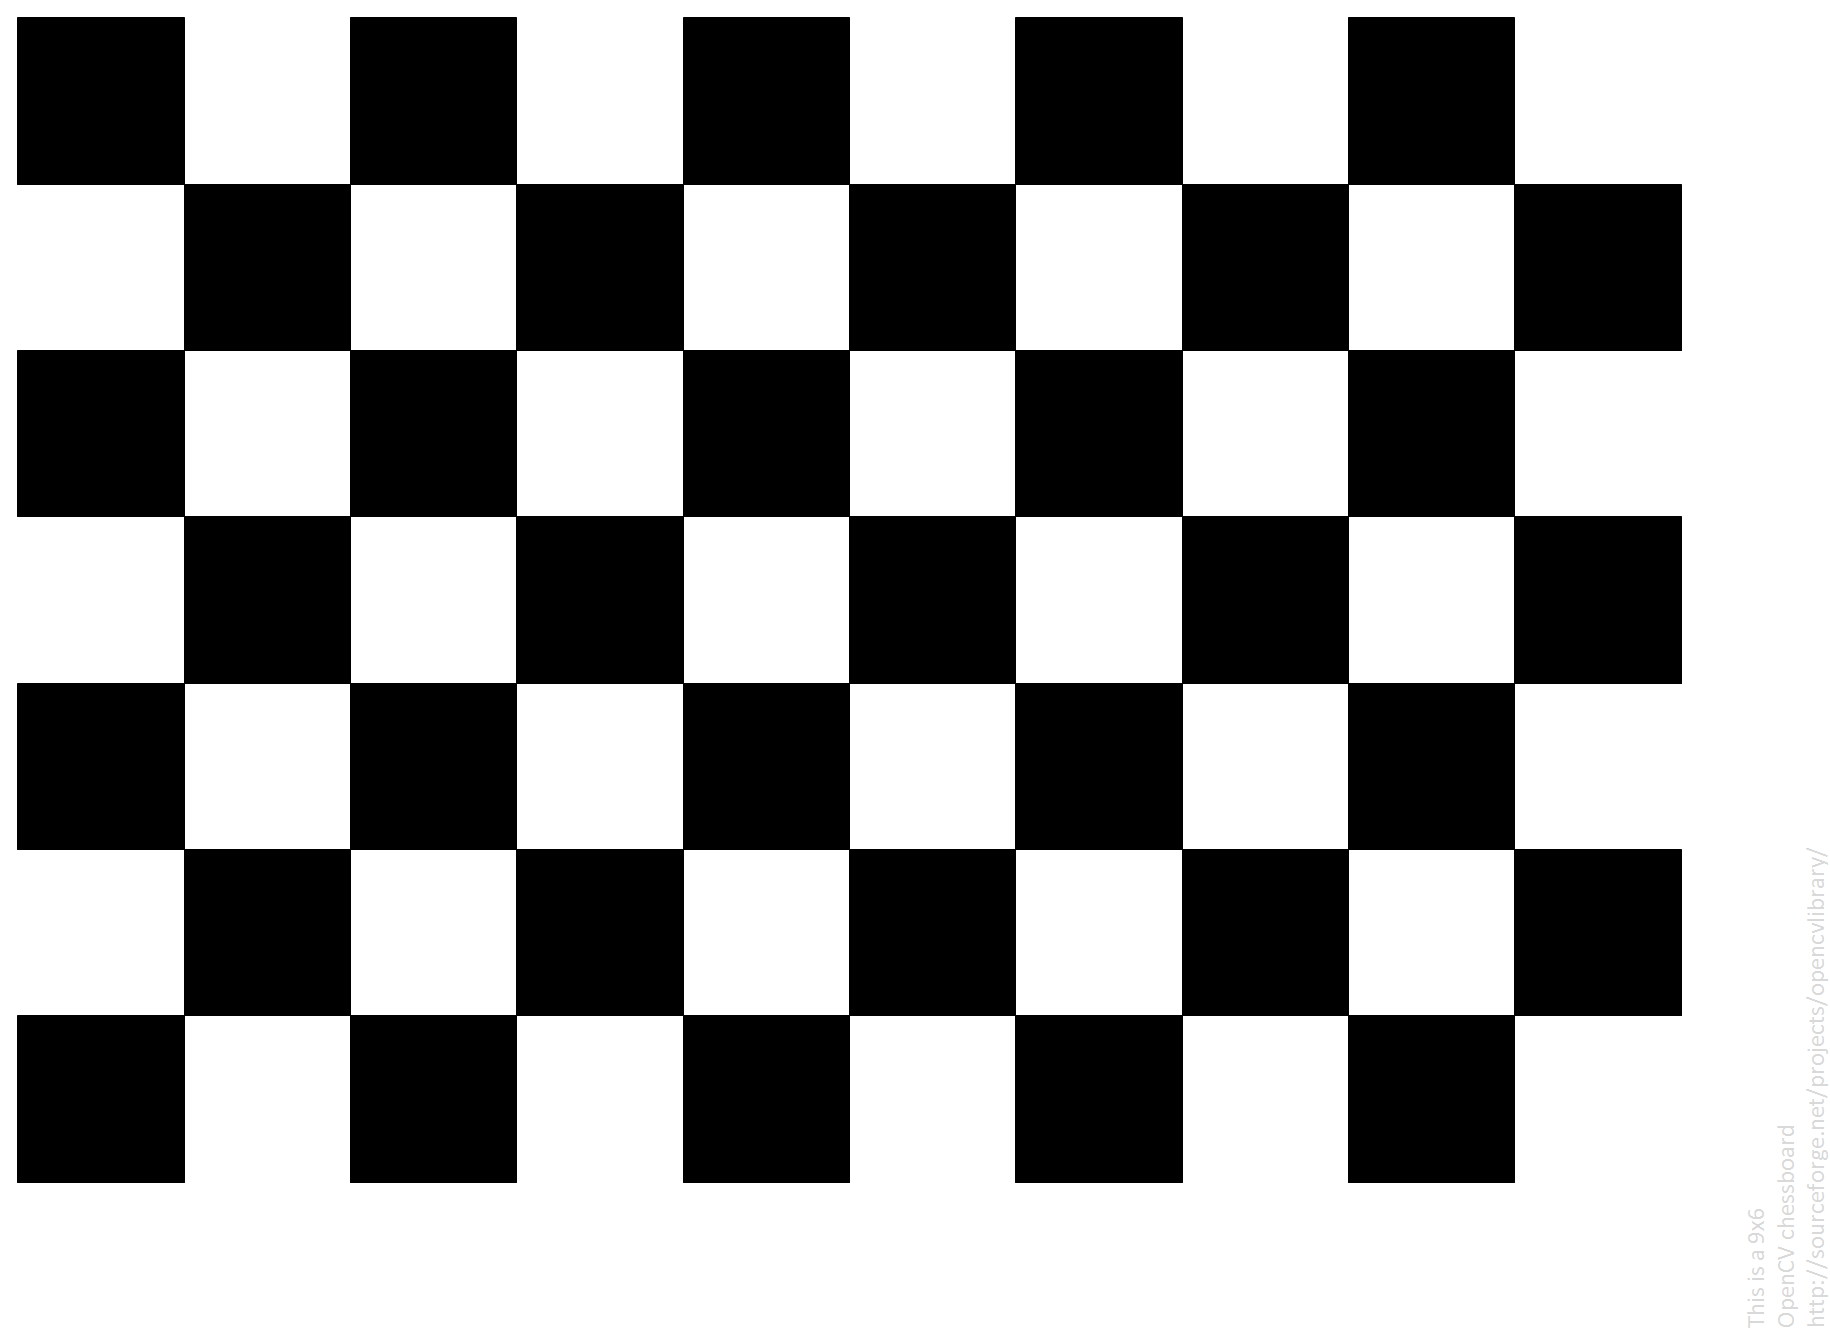
\includegraphics[scale= 0.25,clip]{images/pattern}
\caption{Example of Coordinates Frame Pattern}
\label{fig:pattern}
\end{figure}
\item At Matlab, the images must be added to the toolbox, for this example 40 images were added.
\item The toolbox input is just the size of the square of the pattern (in this case 72 mm).
\item For each image the patter will find the corners of the patter, i.e figure \ref{fig:corners}.

\begin{figure}[ht!]
\centering
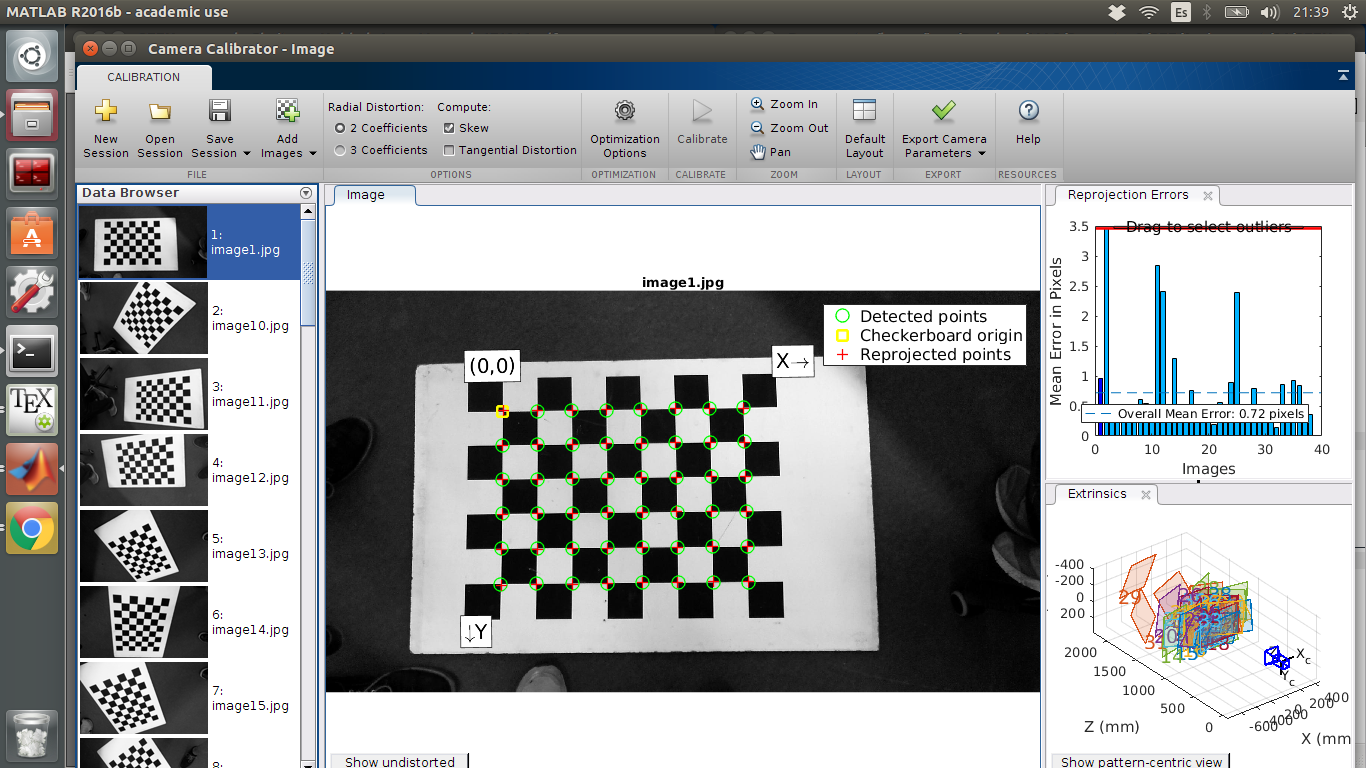
\includegraphics[scale=0.5,trim={350 100 320 300}, clip]{images/borders}
\caption{Border Detection}
\label{fig:corners}
\end{figure}
\item In addition, the toolbox also find the Reprojection Error per Image \ref{fig:errors}
\begin{figure}[ht!]
\centering
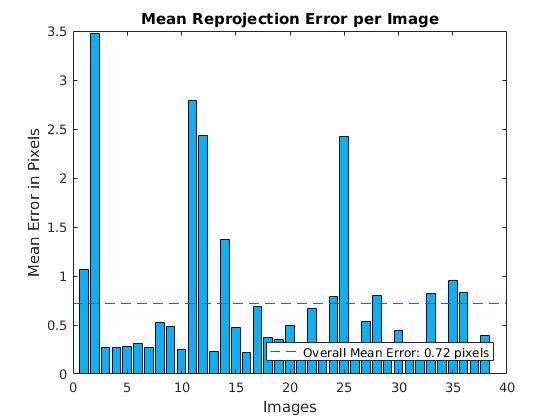
\includegraphics[scale=0.5]{images/errors}
\caption{Mean Reprojection Error per Image}
\label{fig:errors}
\end{figure}
\item The calibration also allow to find the exact location of the pattern for each camera (shown at figure \ref{fig:extrinsic}. It is important to notice that might be a good idea to skip some of the image in order to have an smaller error.
\begin{figure}[ht!]
\centering
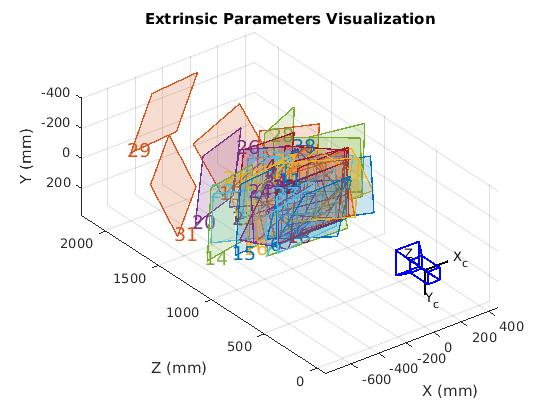
\includegraphics[scale=0.70]{images/extrinsic}
\caption{Extrinsic Parameters Visualization}
\label{fig:extrinsic}
\end{figure}
\end{itemize}

The parameters provided at calibration are shown in the next sections.

\section*{Camera Parameters}

\subsection*{Intrinsic Matrix}
Intrinsic Matrix = \[\left[\begin{matrix}
1460.7&0&0960.9\\
0&1463.9&548.6\\
0&0&1\\
\end{matrix}\right]
\]

Focal length (fx,fy) at pixels are: $[1460.7,1463.9]$\\
Where the principal point coordinates are $[960.9,548.6]$ in pixels.\\
Skew (row 0 col 1) indicates the perpendicularity of the axis of the image plane.\\

\section*{Radial Distortion}

Radial Distortion Coefficients are $[k1 = 0.0063, k2 = 0.0215]$. This coefficients comes from an arbitrary unknown function that is normal modeled by Taylor Expansion the radial distortion model \cite{PerceptionSlides}:

\[
	L(r) = 1 + k_1 r + k_2r^{2}\cdots
\]

Which is used to get the correct coordinates from an image using:

\[
	\hat{x} = x_c + L(r) (x - x_c) 
\]

\[
	\hat{y} = y_c + L(r) (y - y_c) 
\]


Whiere (x,y) are measured coordinates, ($\hat{x},\hat{y}$) are corrected coordinates and ($x_c,y_c$) is the center of the radial distortion. And r is the distance from the center of radial distortion.


\subsection*{Camera Errors}

SkewError: 0\\
FocalLengthError: $[4.1389 4.1263]$\\
PrincipalPointError: $[1.5877 1.4350]$\\
RadialDistortionError: $[0.0046 0.0155]$\\
TangentialDistortionError: $[0 0]$\\

\section*{Experiment Design}

\begin{itemize}
	\item If the position of the camera is known then the problem can be simplify.
	\item With one single camera is not possible in general to locate the position of one point in the camera in world frames, however is possible to obtain a distance to it if the size of the object is known.
	\item Having the focal length, the pixel where is the center of the camera could be known.
	\item Taking one point to calculate the distance in pixels can be known.
	\item A scale factor could be calculated if the area or size of the object is known, then multiplied this factor to the distance in pixels a distance from principal point in longitude is obtained.
	\item It can be transformed using a Homogeneous transform to the World Frame.
\end{itemize}

\section*{Possible Problems}

\begin{itemize}
	\item The size of the marker must be known to estimate scale factor.
	\item Detection of the marker could be an issue if the illumination is not optimal.
	\item Accuracy of measurement relies on the quality of the calibration.
\end{itemize}


\begin{thebibliography}{X}
\bibitem{MatlabDoc} \textsc{Matlab Documentation}
\href{https://de.mathworks.com/help/vision/examples/evaluating-the-accuracy-of-single-camera-calibration.html#zmw57dd0e4306}{Link}
\bibitem{MatlabDoc} \textsc{Robot Perception Course Slides}. Prof. Paul Pl\"oger. Hochschule Bonn Rhein Sieg..
\end{thebibliography}


\end{document}